\section{Related Work} 
\label{sec:related_work}

Much work has been previously done in the field of bike share systems. The research conducted on this topic were primarily of two kinds. First, we found that most of the research journals and conference papers about bike-sharing systems focused on the design aspect of these systems, leaning more towards its functionality and working rather than focusing on developing novel visualizations to better represent this data. These research articles did have visualizations of the bike share data but the analysis from the visualization was ultimately used to support or reinforce the original topic of the research. One of the earliest studies in the idea of bike-sharing by DeMaio \cite{DeMaio:2009:MetroBike} talks about the history of bike-sharing and the potential future of this kind of a system. The article while lacking in the visualization aspect gives a strong concept of the bike-sharing system by also talking about the costs and business model of such a system. Though our project leans more towards the visualization aspect of data, these studies give a sound background knowledge to your subject matter. 

Fishman does a more robust study of this system \cite{Fishman:2016:BikeShare} by working on the bike-share data to analyze a considerable number of ideas such as user preference, user frequency, trip purpose, rider demography, and correlation with the health of the rider. This detailed study also looks into ideas for managing and expanding the bike-share system for future use. Combining simple visualizations with detailed analysis, this paper helped in giving us ideas about possible analysis to perform on our own project. 
\begin{figure}[h]
	\centering % avoid the use of \begin{center}...\end{center} and use \centering instead (more compact)
	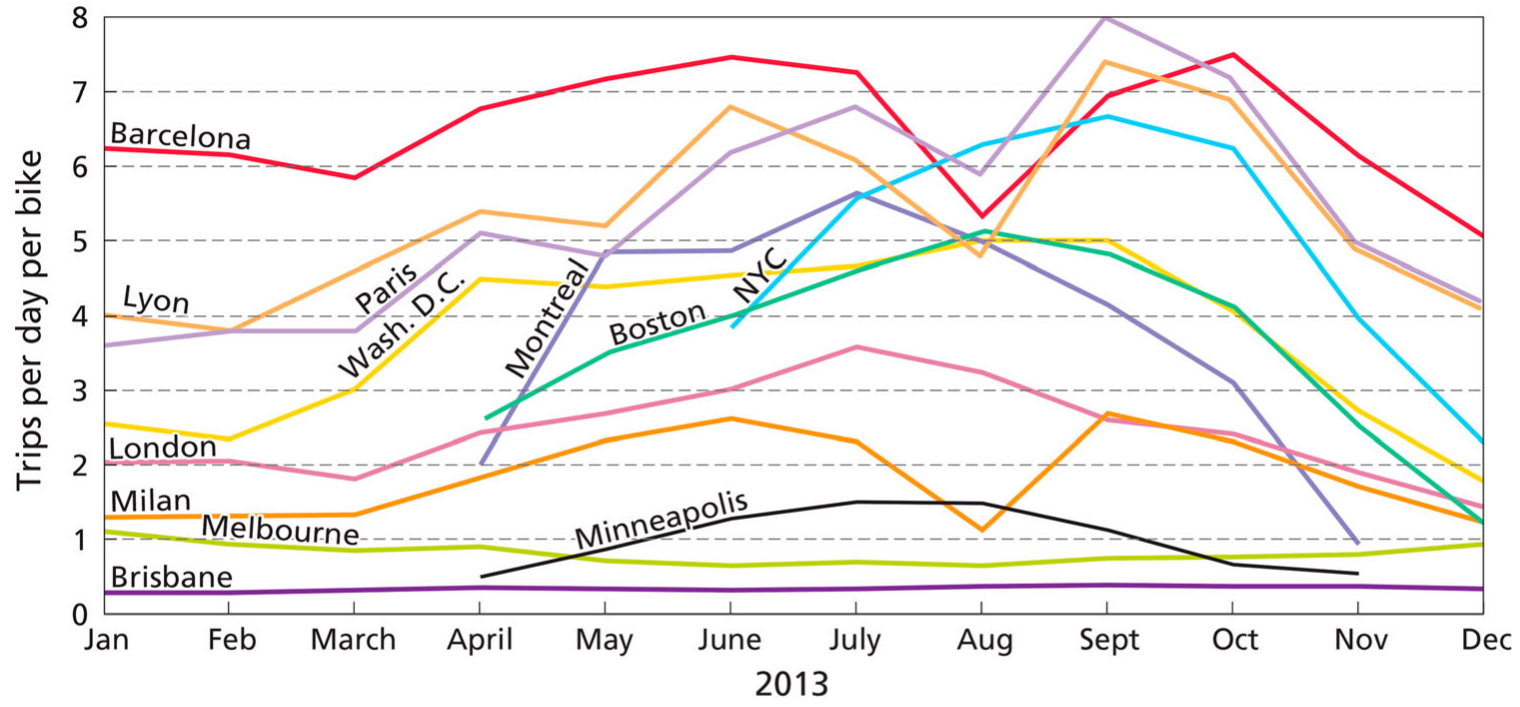
\includegraphics[scale=0.25]{figs/bikeshare_lit1.PNG}
	\caption{\footnotesize{Bikeshare usage, trips per day, per bike, 2013. \cite{Fishman:2016:BikeShare}}}
	\label{fig:Line Chart}
	\captionsetup{justification=centering,margin=1cm}
	\vspace{-10pt}
\end{figure}
\newline
A similar research conducted on university students \cite{Garcia:2015:Univ} studies the effect of using bike-sharing systems on the student's health. Though health is a recurring concept that comes with bike-sharing, our project does not delve into the effect of bike-sharing on the health of riders. By considering the number of calories burnt from each ride, the idea of health can be a topic for future study and expansion of this project. Along the same line of this, a research by DeMaio and Gifford \cite{DeMaio:2004:Success} questions if the bike-sharing system will be successful in the United States. The paper looks into various aspects that would make a bike-sharing system successful such as customer demand, bike facilities, theft and vandalism, profitability and connectivity. It concludes that while such a system might not be feasible in every city in the United States, well-planned consideration of the location can result in this system being successful. This again was a more theoretical approach to the bike-sharing idea rather than involving visualizations.

Coming now to the second type of research on the topic of bike-sharing, we found a lot of standalone visualizations for these datasets. One of the primary reasons for this is because bike-sharing data is easily available online and is free to use by anybody \cite{KaggleData, BikeShareMetro}. This makes it a common source of data for various visualization projects. One visualization study \cite{BayAreaViz} that follows the same direction as our project took the bike-sharing data of the bay area and used Shiny to perform a number of visualizations on it. Using almost all the attributes provided by the dataset, this study created visualizations for a number of sub-topics such as station use frequency, path frequency, bike usage direction, and customer types. Though our project focuses only on a single visualization design, this kind of extension can give the direction for future enhancements. This study also correlates weather data with bike-sharing data to find some relation between the temperature during the day and the rate if bike usage. This is something our project will include as an optional milestone if time persists.
\begin{figure}[h]
	\centering % avoid the use of \begin{center}...\end{center} and use \centering instead (more compact)
	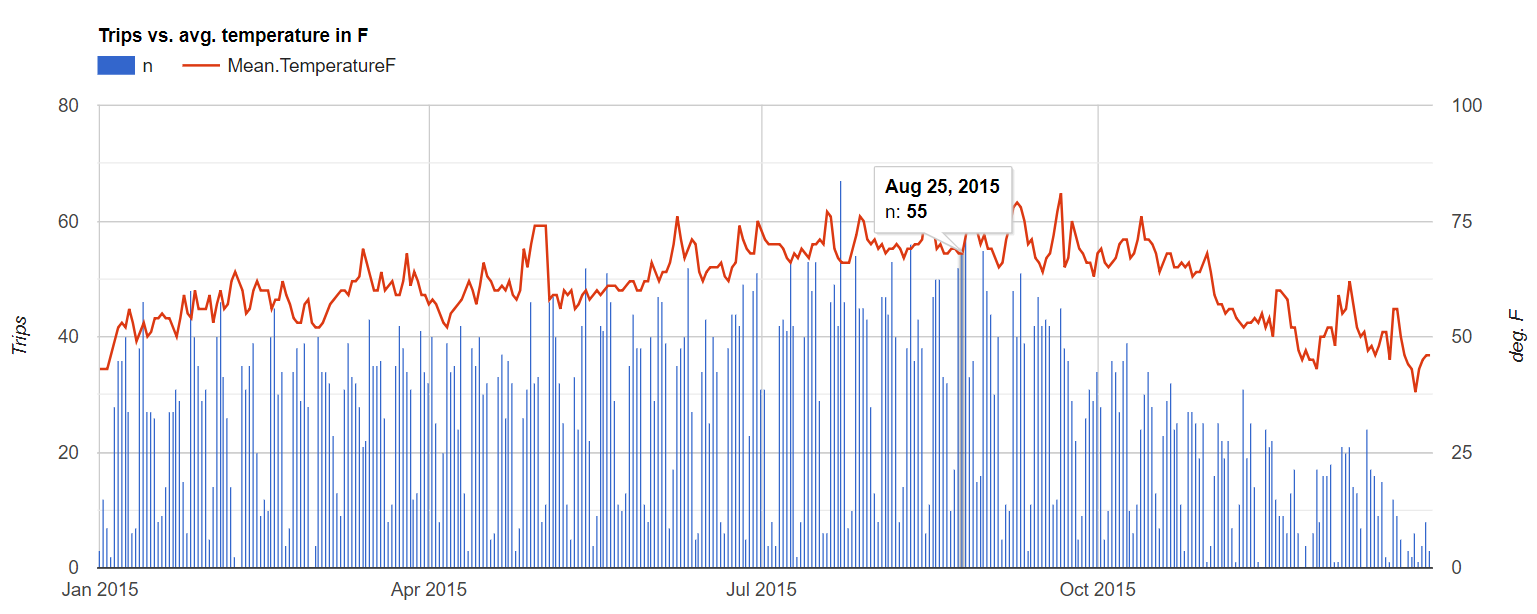
\includegraphics[scale=0.26]{figs/temp.PNG}
	\caption{\footnotesize{Mapping of trip data vs the average temperature. \cite{BayAreaViz}}}
	\label{fig:Weather Chart}
	\captionsetup{justification=centering,margin=1cm}
	\vspace{-10pt}
\end{figure}
\newline
Mobility Lab \cite{MobilityLab} studied the rider behavior of member riders and casual riders and examined stark differences between their riding patterns. This study had a GPS transmitter attached to each bike which allowed them to map actual paths taken by each bike. Having the ability to map actual paths open up a wide variety of possible visualization options to choose from.
\newline
\begin{figure}[h]
	\centering % avoid the use of \begin{center}...\end{center} and use \centering instead (more compact)
	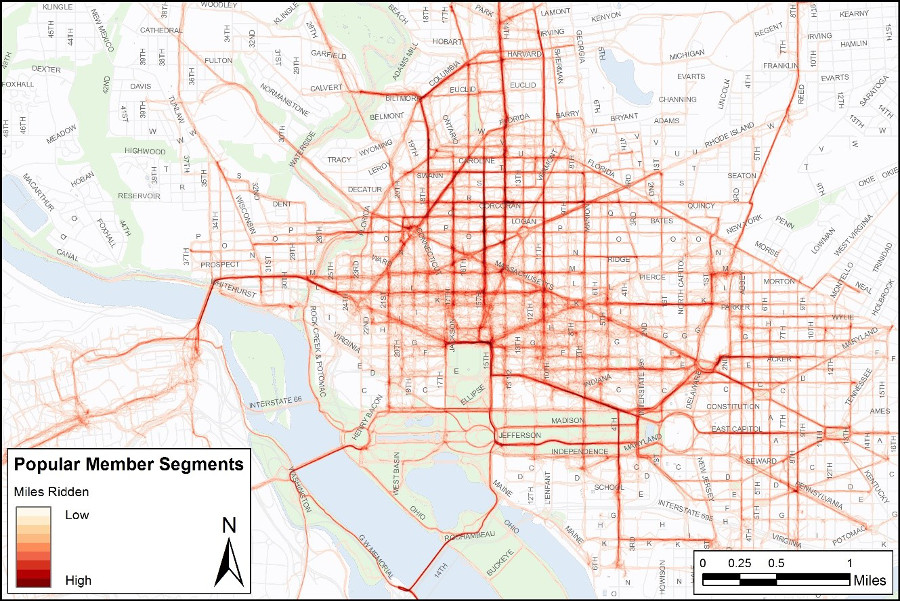
\includegraphics[scale=0.8]{figs/Member-segments.jpg}
	\caption{\footnotesize{Travel paths for trips by members of the bike-share club. \cite{MobilityLab}}}
	\label{fig:Path Chart}
	\captionsetup{justification=centering,margin=1cm}
	\vspace{-10pt}
\end{figure}
\newline
The data for our project does not have the path coordinates so this kind of visualization will not be implemented in the project. In addition to these tools and experiments, there are some research papers that combine data analysis with a strong visualization implementation. Such a research conducted by Zamir, Shafahi and Haghani \cite{shafahi:2017:UVBSDB} studies the imbalance in bike quantity in different locations of a city. They used data mining techniques such as clustering for grouping the bike-sharing stations that have similar temporal activity patterns regarding pickups and drop-offs along with visualization. They argue that the results of this grouping can be used as a tool for analyzing the balancing efforts needed, and improving the design of stations. This paper was a source of unique insight into the bike-sharing system and provided us different ways in which problems can be perceived and solved.
\begin{figure}[h]
	\centering % avoid the use of \begin{center}...\end{center} and use \centering instead (more compact)
	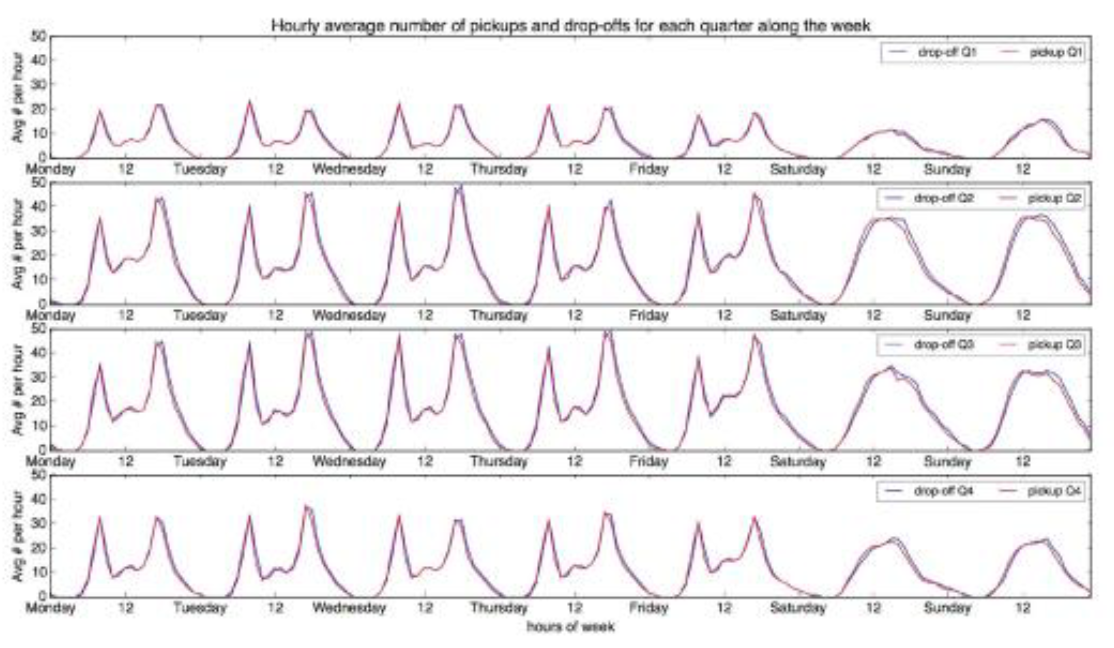
\includegraphics[scale=0.35]{figs/hourly_bike.PNG}
	\caption{\footnotesize{Hourly average of pickups and drop-offs along different hours of the week per quarter. \cite{shafahi:2017:UVBSDB}}}
	\label{fig:Hour Chart}
	\captionsetup{justification=centering,margin=1cm}
	\vspace{-20pt}
\end{figure}
\newline